\section{Tested chains and the classification reduction}
\label{sec:classification}
\label{cls:section}

All constants called absolute in this section are independent of the finite
group, the lattice, the Lie rank, the characteristic, the field degree, and
the length of the chain.  A bound depending on a fixed rank bound is stated
as such.  We use the labels and factor transport of
Lemma~\ref{frm:labels} and Proposition~\ref{frm:active-transport}.

For $k\ge2$, write $M_k$ for the height-two lattice with $k$ atoms;
thus $M_{16}$ has eighteen elements.

\begin{definition}[A tested chain]\label{cls:tested-chain}
Let $D<a<b$ belong to a finite group interval, and let
\[
 a=x_0<x_1<\cdots <x_N=b.
\]
A tested chain consists of these vertices and vertices $v_{ij}$ for
$0\leq i<j\leq N$, with the following properties.
\begin{enumerate}[label=\textup{(T\arabic*)},ref=T\arabic*]
\item\label{cls:test-labels}
Every $x_i$ and $v_{ij}$ is labelled: its interval above $D$ is fenced.
Moreover, $x_i\prec v_{ij}\prec x_j$, where both relations are covers in
the entire interval.
\item\label{cls:test-fences}
Every $[x_i,x_j]$, $i<j$, is fenced.
\item\label{cls:test-saturation}
Every $x_i$ with $i<N$, and every $v_{ij}$ with $j<N$, is an intersection
of coatoms of $[a,b]$.  The $v_{iN}$ are coatoms by
\ref{cls:test-labels}.
\item\label{cls:test-alternating}
Put
\[
 \mathcal U=\{x_j:1\leq j\leq N\}
 \mathbin{\cup}\{v_{ij}:1\leq i<j\leq N\}.
\]
For each $u\in\mathcal U$, the interval $[a,u]$ is fenced, $a$ is an
intersection of its coatoms, and there is $a<c_u<u$ such that the
\emph{entire} interval $[c_u,u]$ is $M_{16}$.
\item\label{cls:test-normal}
For $i<j$ and $x_i\leq z\leq x_j$, either $[D,z]$ is fenced, or there is
a labelled $z'$ with $x_i\leq z'<z$ which is comparable with every vertex
of $[D,z]$.
\end{enumerate}
No additional requirement is imposed on $[a,v_{0j}]$.  In particular,
\ref{cls:test-alternating} never subdivides the cover $a\prec v_{0j}$.
\end{definition}

Condition~\ref{cls:test-normal} ensures the following consequences at
every overgroup between chain vertices: every soluble normal subgroup
is contained in $D$, and, of two normal subgroups whose commutator
lies in a normal subgroup contained in $D$, at least one is contained
in $D$.  At a fenced vertex these follow from Lemma~\ref{frm:labels};
at a labelled bottleneck they follow from
Corollary~\ref{frm:bottleneck}.  The same consequences hold modulo a
higher labelled core, which is normal in each intermediate vertex
and contained in $D$.  No full supplementation dichotomy at an
unlabelled bottleneck is asserted.
The construction in Section~\ref{sec:lattices} will verify exactly
Definition~\ref{cls:tested-chain}.
Figure~\ref{fig:tested-chain} isolates the shortcut comparison; the
remaining tests make this comparison effective uniformly over finite groups.
\begin{figure}[htbp]
\centering
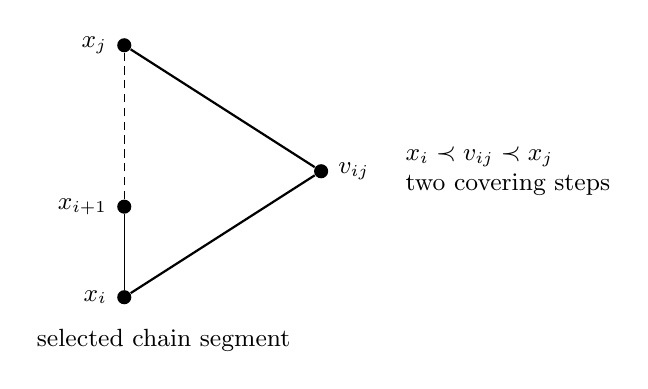
\begin{tikzpicture}[x=1cm,y=1cm,
  vertex/.style={circle,fill=black,inner sep=1.8pt},
  every node/.style={font=\small}]
\node[vertex,label=left:{$x_i$}] (lo) at (0,0) {};
\node[vertex,label=left:{$x_{i+1}$}] (mid) at (0,1.15) {};
\node[vertex,label=left:{$x_j$}] (hi) at (0,3.2) {};
\node[vertex,label=right:{$v_{ij}$}] (shortcut) at (2.5,1.6) {};
\draw (lo)--(mid);
\draw[densely dashed] (mid)--(hi);
\draw[thick] (lo)--(shortcut)--(hi);
\node[align=left,anchor=west] at (3.45,1.6)
  {$x_i\prec v_{ij}\prec x_j$\\two covering steps};
\node[align=center] at (0.5,-.55) {selected chain segment};
\end{tikzpicture}
\caption{One shortcut in a tested chain. The two thick edges are covers
in the entire subgroup interval; the selected chain on the left can
have arbitrarily many intermediate vertices and is not required to be
saturated. Fences, coatom witnesses, and the $M_{16}$ tests are omitted.
The proof compares the restrictions imposed by every short route with
those imposed by traversing a long chain.}
\label{fig:tested-chain}
\end{figure}


\begin{theorem}[Chain rigidity]\label{cls:chain-rigidity}
There is an absolute integer $B$ such that every tested chain of length
$N\geq B$ satisfies $T_a\cong T_b$.
\end{theorem}

The proof proceeds by contradiction through arbitrarily long tested
chains whose endpoint types differ.  This section gives the classification
and uniformity reductions.  Proposition~\ref{grw:remaining-paths} removes
the geometric and cross-characteristic alternatives; the proof of
Theorem~\ref{cls:chain-rigidity} is completed in Section~\ref{sec:rigidity}.
Passing to a subchain always retains the originally supplied shortcuts
and tests.  It does not assert that the subchain, with a new initial
endpoint, is a new tested chain.

\subsection{Literature inputs and maximal-step factor actions}

\begin{proposition}[Maximal-subgroup input]\label{cls:literature}
The following results are used from the classification and representation
theory of finite simple groups.
\begin{enumerate}[label=\textup{(L\arabic*)}]
\item A maximal subgroup of an almost simple classical group, not
containing its socle, is a stabilizer in one of Aschbacher's eight
geometric collections, or has an almost simple irreducible component.
The geometric collections are subspace or flag stabilizers, direct-sum
decompositions, extension-field structures, tensor products, subfield
structures, symplectic-type groups, tensor-induced decompositions, and
forms.  Graph automorphisms may interchange the relevant subspaces or
flag members; triality and exceptional graph--field automorphisms occur
only in bounded rank.  We use
\cite{Aschbacher1984} and the almost simple formulation and descriptions
in \cite[Table~1.2.A and Theorem~1.2.1, pp.~3--4]{KleidmanLiebeck1990},
with the geometric descriptions in Chapters~3--5; the connected tensor
structures and their finite fixed-point versions are also given in
\cite[Theorem~2 and Section~4(5)]{LiebeckSeitzClassical1998}.
\item The maximal subgroups of alternating and symmetric groups have
the intransitive, imprimitive, affine, diagonal, product-action, or
almost simple alternatives of the maximal-subgroup form of the
O'Nan--Scott Theorem.  The relevant formulation and all the alternatives
used here are recorded in the proof of
\cite[Proposition~3.1]{BurnessLiebeckShalev2017}.
\item For a fixed algebraic type, sufficiently general finite subgroups
lie between the derived group and the inner-diagonal group of a finite
fixed-point group.  The complementary alternative is containment in a
proper algebraic subgroup of bounded complexity.  The bounded-envelope
version permits passage to the reductive simple quotients of that
subgroup; see \cite[Theorems~0.5 and~12.3]{LarsenPink2011}.
\item A subgroup maximal in a maximal subgroup of an almost simple
group has at most five nonabelian chief factors
\cite[Proposition~8.1]{BurnessLiebeckShalev2017}.  The number refers to
chief factors, not to their simple direct factors.
\item If $[H,A]$ is a height-two interval and $A$ is alternating or
symmetric of degree at least five, it has at most eleven interior
vertices \cite[Theorem~D]{Basile2008}.  Here the entire interval is required to have height two: $H$ is
maximal in every maximal overgroup. This is the hypothesis imposed
whenever the result is used.
\item Cross-characteristic irreducible projective degrees satisfy the
Landazuri--Seitz lower bounds \cite{LandazuriSeitz1974}.  In particular,
outside bounded rank, a source of natural dimension $n$ and field parameter $q$ requires
degree at least $q^{c n}$ for an absolute $c>0$; the applicable
classical bounds are recorded in \cite[Tables~3--6]{Hasa2014}.
Above an absolute classical rank, every perfect central cover of a
finite simple classical group is a central quotient of its usual
simply connected fixed-point group, uniformly over all finite fields,
including the standard graph twists
\cite[Theorem~1.1 and p.~528]{Steinberg1981}.
The central-cover deduction and preservation of representations
are proved in Lemma~\ref{lift:finite-covers}.
After passing to that cover, defining-characteristic irreducibles
have the Steinberg highest-weight and tensor-product parametrization
\cite[Theorems~1.1 and~1.3]{Steinberg1963}, including the twisted
fixed-point groups \cite[Theorem~43]{SteinbergNotes}.
\end{enumerate}
\end{proposition}

The clauses of Proposition~\ref{cls:literature} are literature inputs.
We first control the actions on simple factors and the resulting chains
of projected cores. Numerical field and dimension estimates will enter in
Section~\ref{grw:section}, after the reduction obtained here. No classification of arbitrary subgroup
chains is assumed.

For a transitive action of a group $K$ on a factor set, with point
stabilizer $K_\omega$, a tower
$K_\omega=K_r\leq\cdots\leq K_0=K$ describes successive invariant
block systems. We call the induced coset actions of $K_{j-1}$ on
$K_{j-1}/K_j$ its \emph{action levels}. The action kernels remain in
these stabilizer groups.

\begin{proposition}[Factor actions at a maximal step]\label{cls:factor-actions}
Consider a strict labelled cover and its one-coordinate maximal subgroup
$M$ in an almost simple group, as supplied by
Proposition~\ref{frm:projection}. Mark its active nonabelian chief factor.
There are absolute positive integers $b_0,r_0$ with the following property.
\begin{enumerate}[label=\textup{(C\arabic*)}]
\item\label{cls:cat-actions}
The action on the simple factors of the marked chief factor is obtained
through at most $r_0$ transitive action levels.  Each level either has
degree at most $b_0$, or is the natural action of $A_d$ or $S_d$.
\end{enumerate}
\end{proposition}

\begin{proof}
We spell out the factor actions.  A subspace or paired-flag
stabilizer has at most a bounded number of Levi components.  A tensor
product of two spaces has two component groups.  Extension-field,
subfield, form, and almost simple cases have one, except for the
bounded low-dimensional coincidences.  A direct-sum decomposition or
a tensor-induced decomposition has the full symmetric action on its
blocks, with a possible alternating restriction from the determinant
or spinor condition.  A block contributes at most a bounded number of
simple factors; for instance an orthogonal plus-type four-space
contributes two.  Taking a point inside a block and then the block
itself accounts for this extra bounded level.  In the alternating
case, the intransitive and affine alternatives have bounded component
actions, while the imprimitive, diagonal, and product-action
alternatives have this same full block action.  Exceptional types have
bounded rank and hence bounded numbers of components.  Central,
determinant, and form quotients do not split a simple component into
more factors.  This proves \ref{cls:cat-actions}; the explicit
$\mathcal C_2$ and $\mathcal C_7$ component quotients can also be read
in \cite[proofs of Lemmas~5.4 and~5.9]{BurnessLiebeckShalev2017}.
\end{proof}

Several structural consequences of the maximal-subgroup descriptions
will be needed when we reduce to classical groups of large rank.
For a classical target and a classical active source type of sufficiently
large rank, a cover with more than one active simple factor belongs to the
geometric block or tensor cases. A soluble classical component has absolutely
bounded natural dimension: a linear group in growing dimension contains
a growing special linear simple section, and the corresponding assertion
for a form group follows from its natural hyperbolic subspaces.
For a fixed nonabelian simple type, the possible natural classical
realizations have boundedly many dimensions. Outside the bounded list
of low-order isomorphisms, its field, family, and dimension are determined
by its type; dual, form, and special-isogeny conventions add only
boundedly many choices. Finally, a geometric stabilizer has boundedly
many component slots apart from repeated blocks. Thus fixing the inactive
simple labels, repetition degrees, and bounded structural choices leaves
boundedly many possible omitted dimensions. These facts use the full
geometric stabilizers in Proposition~\ref{cls:literature}(L1), not a bound
on the orders of the components. Their numerical field and order data
will be established in Section~\ref{grw:section}.

\subsection{A uniform lemma for natural giant actions}

The shortcuts will put the relevant factor stabilizers inside one fixed
projected bottom group. We need to control their composition types and
indices simultaneously. The next two lemmas do this for bounded
stabilizer towers, including the overgroups that arise when equal-type
strips are merged.

For a finite group $H$, write $\operatorname{cf}_{\mathrm{na}}(H)$
for its set of nonabelian simple composition-factor types.  Only these
types will be bounded; the set of cyclic-prime factors need not be.

\begin{lemma}[Bounded routes]\label{cls:routes}
Fix positive integers $r,b$.  Suppose
\[
 A=H_r\leq H_{r-1}\leq\cdots\leq H_0=H
\]
and every induced action on $H_{j-1}/H_j$ is either of degree at most
$b$ or is a natural alternating or symmetric action.  There are
constants $h,c,k$, depending only on $r,b$, such that:
\begin{enumerate}[label=\textup{(\roman*)}]
\item the interval $[A,H]$ has height at most $h$;
\item the set $\{[H:U]:A\leq U\leq H\}$ has cardinality at most $k$;
\item for every such $U$, its nonabelian composition types belong to
\[
 \operatorname{cf}_{\mathrm{na}}(H)
 \cup\{A_{d-j}:A_d\in\operatorname{cf}_{\mathrm{na}}(H),\ 0\leq j\leq c\}
 \cup\mathcal E_{r,b},
\]
where $\mathcal E_{r,b}$ is a fixed finite set of types.
\end{enumerate}
The conclusions also hold for stabilizers of all invariant quotient
blocks of the action on $H/A$.
\end{lemma}
\begin{proof}
We induct on $r$.  The assertion for one step follows from primitivity
of a natural giant, or from the bounded index in the other case.
For the induction put $N=\operatorname{core}_H(H_1)$.  For an
arbitrary $U\in[A,H]$, the group $A(U\cap N)$ lies in $[A,H_1]$,
and its intersection with $N$ is $U\cap N$.  The induction hypothesis
therefore controls the intersection chain and its types.  A strict
increase in $U$ must increase $U\cap N$ or $UN/N$, since equality of
both gives equality of orders.  Furthermore
\[
 [H:U]=[H/N:UN/N]\,[N:U\cap N],
\]
and the possible second factors are a fixed multiple of the possible
indices $[H_1:A(U\cap N)]$.  Thus it remains to control the images.

If $H/N$ has bounded degree, its order is at most $b!$ and there is
nothing more to prove.  Otherwise it is $A_d$ or $S_d$, and $H_1/N$
is its natural point stabilizer.  Project the remaining route into
$H_1/N$.  A natural-giant step projects either to the same action or
to a trivial action, because it is primitive; a bounded-degree step
retains bounded degree.  Starting with the natural $A_{d-1}$ in
$H_1/N$, retain an alternating group normal in the current projected
group and supported on all but at most $r$ points.  A natural-giant
quotient either kills this alternating group, which is then retained
in the next subgroup, or maps it onto the natural alternating socle
of its image.  In the latter case equality of orders gives the same
degree, and its point stabilizer removes one supported point.
A step of bounded degree retains the alternating group once its
order exceeds $b!$.  After a step, take the union of all conjugates
of the retained support in the new subgroup.  The overlapping-support
argument in the next paragraph supplies a normal alternating group
on that union, without further loss of points.
Apart from a possible sign on the large support, the residual
quotient acts on the omitted points and has order at most $2r!$.
For $d>2r+b+10$, each step therefore loses at most one supported
point, and the terminal image contains the alternating group
supported on at least $d-r$ points.  Here the identification
of the next point stabilizer uses
$\operatorname{Aut}(A_e)=S_e$ for $e\geq7$; the degree-six exception
and all smaller first degrees are absorbed in the fixed finite
universe.  Thus we may take $c=r$ in the large-degree argument.

An overgroup of an alternating group supported on $d-c$ points has
bounded height and boundedly many possible indices.  To see this
directly, assume $d>2c+4$.  The supports of any two conjugates overlap
in at least three points, so their alternating groups generate the
alternating group on the union of their supports.  The union of
all conjugate supports is an orbit of the overgroup; its conjugate
alternating groups generate the alternating group on that orbit.
The orbit omits at most $c$ points.  Modulo the
alternating group on that orbit, the overgroup has order at most
$2c!$.  Its large simple type is therefore $A_{d-j}$ with
$0\leq j\leq c$, and its possible indices belong to the finite list
of falling factorials $(d)_j$ divided or multiplied by integers
bounded in terms of $c$.  The excluded small $d$ add only bounded
groups.  Combining this with the intersection induction proves
all three conclusions.  Invariant quotient blocks correspond
exactly to the overgroups $U$ already considered.
\end{proof}

\begin{lemma}[A common index palette]\label{cls:index-recipes}
Fix positive integers $R,b,K$.  Consider any collection of the
routes in Lemma~\ref{cls:routes}, each of length at most $R$ and
bounded degree at most $b$, such that all their natural giant
degrees belong to one set $\mathcal D$ with $|\mathcal D|\leq K$.
The union, over all groups and routes in the collection, of all
indices $[H:U]$ with $A\leq U\leq H$ has cardinality bounded by a
function of $R,b,K$.  The same holds through a bounded number of
operations, each consisting of a permitted route followed by an
arbitrary invariant quotient-block choice, with a fresh route
inside the chosen block stabilizer permitted at the next operation.
\end{lemma}
\begin{proof}
Put $d_0=2R+b+10$ and $M=d_0!$, and define the positive rational
atoms
\[
 \Gamma(\mathcal D)=
 \{u/v:1\leq u,v\leq M\}
 \cup\{(d)_j:d\in\mathcal D,\ d>d_0,\ 0\leq j\leq R\}.
\]
We claim that every index on a route of length $r$ is a product of
at most $L_r=r(r+3)/2$ atoms or their inverses.  Induct on $r$,
putting $N=\operatorname{core}_H(H_1)$ and
$B=A(U\cap N)$.  Since $U\cap N\trianglelefteq U$, we have
$A\leq B\leq H_1$ and $B\cap N=U\cap N$.  Consequently
\begin{equation}\label{cls:route-index-identity}
 [H:U]=[H/N:UN/N]\,
        \frac{[H_1:B]}{[H_1:AN]}.
\end{equation}
The image factor is bounded by $M$ when the first action is small.
Otherwise the supported alternating-group calculation in
Lemma~\ref{cls:routes} gives
\[
 [H/N:UN/N]=\frac{\varepsilon(d)_j}{t},\qquad
 0\leq j\leq r,\quad \varepsilon\in\{1,2\},\quad1\leq t\leq2j!.
\]
It therefore uses at most two atoms.  The numerator $[H_1:B]$
uses at most $L_{r-1}$ atoms by induction.

The denominator is controlled across the whole collection, not
just held fixed within one route.  Project the suffix route into
$H_1/N$.  Its degree is exactly
\begin{equation}\label{cls:route-denominator}
 [H_1:AN]=\prod_{j=2}^{r}
 [H_{j-1}N/N:H_jN/N].
\end{equation}
Under any homomorphism with kernel $C$, a natural step $L_0>L_1$
projects to the same full natural action or to a trivial action:
maximality gives $L_1C=L_1$ or $L_0$.  A bounded step keeps bounded
degree.  Thus every factor on the right of
\eqref{cls:route-denominator} is an allowed natural degree, a
bounded integer, or one, and is a single atom.  In particular no
arbitrary scalar-kernel divisor enters the denominator.
Equation~\eqref{cls:route-index-identity} gives
$L_r\leq L_{r-1}+2+(r-1)$, proving the claim.

There are at most $M^2+K(R+1)$ atoms, so the union of all index
palettes has cardinality at most
\[
 \bigl(1+2(M^2+K(R+1))\bigr)^{L_R}.
\]
Only integral values of these rational recipes occur as actual
indices.  Invariant quotient blocks correspond to the overgroups
$U$ already allowed.  If $H'$ is any such block stabilizer, apply
the argument anew to the next full route inside $H'$; it is not
necessary that $H'$ itself admit a natural-step route from $H$.
Indices multiply through a bounded number of these operations,
giving the final assertion.
\end{proof}

\begin{lemma}[Uniform active actions]\label{cls:uniform-actions}
Suppose a tested chain has $T_a\not\cong T_b$, and project at one
coordinate of the socle of $b$.  Let $H_*$ be the image of the factor
stabilizer in $a$.  Then:
\begin{enumerate}[label=\textup{(\roman*)}]
\item $H_*$ has at most five nonabelian chief factors;
\item there is one set of nonabelian types, of absolutely bounded
cardinality, which contains the types of every whole projected
stabilizer group in $H_*$ of an active factor, of an intermediate
fiber, or of an invariant quotient block used along a two-edge
shortcut, and the types of all their induced images;
\item equal-type stretches of chain vertices have absolutely
bounded length;
\item the set of ratios $m_{x_i}/m_{x_j}$, $i<j$, has absolutely
bounded cardinality after equal-type repetitions are removed.
\end{enumerate}
\end{lemma}
\begin{proof}
By Propositions~\ref{frm:strict-product} and~\ref{frm:projection}, the
starting group is a nontrivial proper coordinate product, and all
designated intersections of coatoms are saturated.  The shortcut
$a\prec v_{0N}\prec b$ projects to a two-step maximal chain in an
almost simple group.  Thus Proposition~\ref{cls:literature} gives
the five-chief-factor bound for the actual projected bottom $H_*$.
The image of the original $D$-stabilizer need not equal $H_*$ as a
group: in general $H_*$ is that image multiplied by the starting
coordinate product.  What is required is equality of the induced
active permutation actions, as follows.

For every label $z$, the equality $z=DN_z$ implies that $D$ and $z$
have the same image on $I_z$, because $N_z$ fixes its individual
simple factors.  If $I_z\to I_w$ is a product-step factor map and
$g\in z$ fixes $i\in I_w$, write $g=dn$ with $d\in D$ and
$n\in N_z$.  Then $d$ fixes $i$ and has the same action as $g$ on
the fiber over $i$.  Thus the bottom stabilizer induces the
\emph{full} local factor action at each level, not an arbitrary
subgroup of the natural giant.  This property survives the initial
projection by Proposition~\ref{frm:active-transport}.

We now account for all the shortcuts, including middles below a
proper endpoint.  An endpoint $x_j$ is reached from $b$ by the
original shortcut $b>v_{jN}>x_j$; take an empty route for $j=N$.
The first downward step is strict, because a proper subdirect group
cannot contain the nontrivial full coordinate product at the bottom.
Two strict covers give a concatenated route of length at most
$2r_0$.  A strict cover followed by an equal-type merge instead
makes the endpoint factor stabilizer an overgroup of the first
route's terminal stabilizer.

Starting at $x_j$, the middle $v_{ij}$ and the lower endpoint $x_i$
are reached by at most two further original covers.  An equal-type
operation takes an invariant quotient block.  A strict operation
supplies a fresh full local route inside the actual current
projected factor stabilizer $U\leq H_*$.  Indeed the image of the
original $D$-stabilizer lies in $U$ and already has the full local
permutation image, whereas $U$ acts through the labelled-node
stabilizer because $a$ lies below that node.  The kernel of the
original-coordinate projection centralizes that coordinate and acts
trivially on its sections.  Thus these are equal local permutation
images; no equality of the stabilizer groups themselves is needed.

The factor maps and equal-type strips respect the original $b$
coordinates.  Here is the intersection identity behind this assertion.
For labels $x\leq z$ used in a route, work modulo $F_b$ and write
\[
 x\cap N_b=P_x^{I_b},\qquad
 N_z\cap N_b=R_z^{I_b},\qquad F_z\cap N_b=Q_z^{I_b}.
\]
These product descriptions follow from saturation and
Proposition~\ref{frm:active-transport}.  Since $F_z\leq D\leq x$ and
$N_z=F_z(N_z\cap N_b)$, intersection and the quotient map give
\[
 \frac{x\cap N_z}{F_z}
 \cong \frac{x\cap N_z\cap N_b}{F_z\cap N_b}
 =\prod_{i\in I_b}\frac{P_x\cap R_z}{Q_z}.
\]
In an equal-type comparison this is the subdirect subgroup of $S_z$
whose strips describe the merge.  Because it is a full product over
$I_b$, no strip can link factors in different original coordinates:
such a link would prohibit independent elements in the two factors.
For a strict split followed by a merge inside $[x_i,x_j]$, repeat this
identity with $x_j$ as upper vertex.  The fenced endpoint comparison
makes $x_i$ saturated in those coordinates, and the strict shortcut
cover makes its middle saturated there.  Thus the merge cannot cross
those local starting fibers either.
Altogether, every required factor, fiber, and quotient-block
stabilizer uses at most four original covers, interpreted as full
local routes or quotient operations.  Four successive operations,
each with route length at most $2r_0$, give a conservative common
bound, including all intermediate block stabilizers.

We establish the type pool before the degree and index pools.  For
fixed route parameters let
\[
 \Phi(\mathcal P)=\mathcal P
\mathbin{\cup}\{A_{d-j}:A_d\in\mathcal P,\ 0\leq j\leq c,\ d-j\geq5\}
\mathbin{\cup}\mathcal E,
\]
where $c$ and the finite exceptional set $\mathcal E$ are supplied
by Lemma~\ref{cls:routes}.  If the whole current projected group has
nonabelian composition types in $\mathcal P$, that lemma puts the
types of every route prefix and every quotient-block overgroup in
$\Phi(\mathcal P)$.  This includes any kernel of the corresponding
permutation action.  Retain the original types at every iteration.
Starting with $\operatorname{cf}_{\mathrm{na}}(H_*)$, of cardinality
at most five, a bounded number of iterations gives one pool of
absolute bounded cardinality for all these projected groups.
Their induced images have no additional composition types.  This
proves (ii); it makes no claim about entire unprojected stabilizers
in the original group.

For an equal-type stretch, fix its highest vertex.  Equal-type
transport identifies all earlier vertices with strip subgroups
of that socle, whose support partitions strictly change along the
stretch.  Equal support partitions and subgroup inclusion would
force equality of orders and hence equality of subgroups, including
the diagonal twists.  The preceding coordinate compatibility
restricts these to invariant partitions of a single original
$b$-coordinate fiber.  Transitivity ensures that a strict change
appears on that chosen fiber.  All their block stabilizers are
overgroups of a single route terminal supplied by the shortcut
from $b$ to the highest vertex.  The height assertion of
Lemma~\ref{cls:routes} proves (iii).

Each full giant of large degree $d$ contributes the composition
type $A_d$ to its actual starting projected group.  Every such group is a route
prefix already covered by the preceding pool.  Hence the set
$\mathcal D$ of giant degree values occurring anywhere in these
bounded operations has absolute bounded cardinality.  The values
may be large.  Apply Lemma~\ref{cls:index-recipes} with this entire
set $\mathcal D$, and multiply indices through the bounded number
of operations.  This yields a common index palette across all the
actions, including arbitrary quotient-block choices followed by
fresh full routes.  In particular it is a union bound, not merely
a separate cardinality bound for each action.

More explicitly, put $q_i=m_{x_i}/m_b$.  The original shortcut from
$b$ to $x_i$ realizes $q_i$ as the degree on its active-factor fiber:
a strict/strict path gives a route degree, and a strict/merge path
gives a quotient-block degree.  The common recipe palette bounds
the cardinality of $\{q_i\}$.  Since
$m_{x_i}/m_{x_j}=q_i/q_j$, its quotient palette also has bounded
cardinality.  This proves (iv).
\end{proof}

\subsection{The core reduction}

\begin{lemma}[Killed layers and core gaps]\label{cls:core-gaps}
In the initial projection, consider chain vertices strictly above the
original starting vertex $a$, and write
\[
 K_i=H_*P_i,\qquad C_i=\operatorname{core}_{K_i}(H_*),
 \qquad Q_i=C_i\cap P_i,
\]
and let $R_i/Q_i$ be its active nonabelian chief factor.  For $i<j$,
the inner comparison and its killed kernel are
\[
 J_{ij}=(P_i\cap R_j)/Q_j,
 \qquad B_{ij}=(Q_i\cap R_j)/Q_j.
\]
There is an embedding $B_{ij}\hookrightarrow C_i/C_j$.
After deleting at most five nonsoluble gaps, an arbitrarily long
subchain remains on which all the $B_{ij}$, including the analogous
shortcut kernels, are soluble.  If the chain multiplicities are
equal, every endpoint inner comparison, projected to one factor of
its upper active socle, has just its active simple factor as a
nonabelian composition factor.
\end{lemma}
\begin{proof}
The exact product/core identity in
Proposition~\ref{frm:active-transport} gives, before projection,
\[
 (F_i\cap N_b)/F_b=Q_i^{m_b},\qquad
 (N_i\cap N_b)/F_b=R_i^{m_b},\qquad
 R_i/Q_i\cong T_i^{m_i/m_b}.
\]
Since $F_j\leq D\leq x_i$, we have $Q_j\leq P_i$.
Intersecting with the lower group and then with its core gives the
displayed formulas for $J_{ij}$ and $B_{ij}$.  Also $C_j\leq C_i$
and $R_j\leq P_j$, whence
\[
 C_j\cap R_j=Q_j.
\]
Thus $uQ_j\mapsto uC_j$ embeds $B_{ij}$ in $C_i/C_j$.

The $C_i$ form a decreasing chain of normal subgroups of the one
group $H_*$.  Each nonsoluble successive quotient consumes at least
one nonabelian chief factor of $H_*$.  There are at most five, by
Lemma~\ref{cls:uniform-actions}.  Cutting at these transitions
leaves at most six stretches; one is arbitrarily long.  The core
of a shortcut middle lies between the cores of its two endpoints,
so its killed layers are controlled by the same soluble quotient.
No separate bound on a collection of unrelated shortcut cores is
being assumed.

For the final assertion work with the original labelled vertices
$x_i<x_j$ and put
\[
 E=x_i\cap N_j,\qquad W=F_i\cap N_j,\qquad L=N_i\cap N_j.
\]
These subgroups are normal in $x_i$, with $F_j\leq W\leq L$.
The kernel of the conjugation action of $E$ on
$S_i=N_i/F_i$ is exactly $W$, because
$C_{x_i/F_i}(S_i)=1$.  When $m_i=m_j$, the product support map
$I_i\to I_j$ is a bijection.  Since $E\leq N_j$ fixes $I_j$,
it fixes every factor of $S_i$.  Its socle preimage is $L$, and
therefore
\[
 E/L\hookrightarrow\operatorname{Out}(T_i)^{m_j},
\]
which is soluble by Schreier's Theorem.  In the $x_j$ coordinates
write
\[
 E/F_j=P_{ij}^{m_j},\qquad W/F_j=Q_{ij}^{m_j},\qquad
 L/F_j=R_{ij}^{m_j}.
\]
Proposition~\ref{frm:active-transport} gives
$R_{ij}/Q_{ij}\cong T_i$, and the preceding embedding makes
$P_{ij}/R_{ij}$ soluble.

The killed kernel is exactly the one controlled in the initial
$b$ projection.  Indeed $N_j=F_j(N_j\cap N_b)$ and $F_j\leq F_i$
give
\begin{align}
 F_i\cap N_j&=F_j(F_i\cap N_j\cap N_b),\label{cls:killed-intersection}\\
 W/F_j&\cong
 \bigl((Q_i\cap R_j)/Q_j\bigr)^{m_b}.\label{cls:killed-kernel}
\end{align}
It is soluble on the retained stretch, so $Q_{ij}$ is soluble as
well.  Thus $P_{ij}$ has exactly its one active simple factor as a
nonabelian composition factor.  The same intersection calculation
identifies the killed kernels for either half of a shortcut.
This argument takes place in the original labelled $x_i$; it uses
neither projected quasiprimitivity nor a supplementation dichotomy
at an unlabelled bottleneck.  A shortcut middle which
still has several active factors can retain a nonabelian
factor-permutation quotient; this is not asserted to be soluble.
Its degrees are controlled by the common type pool, and it occurs
only in the split--merge case considered separately below.
\end{proof}

\begin{lemma}[Exclusion of alternating upper types]\label{cls:alternating}
For $u\in\mathcal U$ with $T_a\not\cong T_u$, the type $T_u$ is
not alternating of degree at least seven.
\end{lemma}
\begin{proof}
Project the strict comparison from $a$ to $u$ using
\ref{cls:test-alternating}.  The bottom is a full product and an
intersection of coatoms.  The coatoms and their intersection $c_u$
are saturated, so Proposition~\ref{frm:projection} carries the entire
interval $[c_u,u]$ to an $M_{16}$ interval ending at an almost simple
group with socle $T_u$.  For an alternating socle of degree at least
seven that group is alternating or symmetric, contradicting
Proposition~\ref{cls:literature}.  The exceptional automorphisms in
degree six concern only bounded-order types.
\end{proof}

\subsection{Why bounded rank cannot support a long strict chain}

The bounded-rank argument needs a normalized subfield group, rather
than just a numerical resemblance between two field sizes.  We give
the details, including the automorphisms of the almost simple ambient
group.

\begin{lemma}[Bounded envelopes]\label{cls:envelopes}
Fix a connected adjoint simple algebraic type $\Phi$.  There is a
constant $c_\Phi$ such that a finite subgroup $P$ of an algebraic
group $X$ of type $\Phi$ has one of the following descriptions.
\begin{enumerate}[label=\textup{(\roman*)}]
\item For a Frobenius map $F_0$,
\[
 E=(X^{F_0})'\leq P\leq X^{F_0},
\]
where $E$ is simple.
\item Every nonabelian composition factor of $P$ of order greater
than $c_\Phi$ is of Lie type in the characteristic of $X$, with
algebraic dimension strictly less than $\dim X$.  The total number
of nonabelian composition factors, counted with multiplicity, is at
most $c_\Phi$.
\end{enumerate}
In particular, the ranks of nonabelian simple sections of finite
groups of Lie type of rank at most $R$ are bounded by a function of
$R$; simple sections of bounded order are included in this bound.
\end{lemma}
\begin{proof}
Apply \cite[Theorem~0.5]{LarsenPink2011}.  Outside (i), $P$ lies in
a proper algebraic subgroup $B<X$ from a fixed constructible family.
Apply \cite[Theorem~12.3]{LarsenPink2011} to that family.  It supplies
an envelope $H\leq B$, with $P\leq H$, whose connected reductive
quotient has simple adjoint factors $X_1,\ldots,X_t$ such that the
image $L_i$ of $P\cap H^\circ$ satisfies
\[
 E_i=(X_i^{F_i})'\leq L_i\leq X_i^{F_i},
\]
with $E_i$ simple.  Each $\dim X_i\leq\dim H^\circ<\dim X$.
The kernel of the map from $H^\circ$ to the product of its simple
adjoint quotients is soluble: it is an extension of the unipotent
radical by the full center of the connected reductive quotient.
That center can be disconnected, but is abelian.  If $L$ is the image of $P\cap H^\circ$
in $\prod_i L_i$, then $L'$ is a subdirect subgroup of
$\prod_iE_i$, because each $L_i/E_i$ is abelian.  The subdirect
product Lemma makes $L'$ a product of full diagonals.  Its simple
factors are therefore among the $E_i$, counted at most once per
position.  There are at most $\dim X/3$ positions.

The component bound in \cite[Proposition~1.4]{LarsenPink2011} bounds
$|H/H^\circ|$ throughout this constructible family.  Its contribution
has bounded order and bounded composition length.  This proves (ii).
Applying the same argument to every subgroup of a finite group of
rank at most $R$ proves the last assertion: the ambient algebraic
dimensions range over a finite set, and the finitely many small
orders and characteristics in the exceptional alternative are
absorbed in a function of $R$.
\end{proof}

\begin{lemma}[Normalized subfield steps]\label{cls:subfields}
Fix an adjoint simple type $\Phi$.  Let $T=(X^F)'$ be simple,
$T\leq A\leq\operatorname{Aut}(T)$, and let $M<A$ be maximal with
$T\not\leq M$.  Suppose that $P=M\cap T$ is in alternative (i) of
Lemma~\ref{cls:envelopes}, and that the parameter of $F_0$ is large
enough in terms of $\Phi$.  Then $F=F_0^r$ for a prime $r$.
Every element of $M$ normalizes the derived fixed-point groups for
all intermediate powers of $F_0$.
\end{lemma}
\begin{proof}
First, the pointwise centralizer of $E=(X^{F_0})'$ in
$\operatorname{Aut}_{\rm alg}(X)$ is trivial when the field parameter
is sufficiently large.  Indeed the fixed groups $X^a$, for nonidentity
algebraic automorphisms $a$, form a constructible family of proper
closed subgroups: take the equalizer of the action and projection
maps over the finite-type algebraic automorphism group, remove the
identity section, and stratify.  Now use
\cite[Proposition~3.5]{LarsenPink2011}.

Here is the isogeny calculation needed to include field and exceptional
graph operations.  Let $\mathcal I(X)$ be the group of bijections of
$X(\overline{\mathbb F}_p)$ generated by self-isogenies and their
inverses.  The isogeny Theorem
\cite[Theorem~6.1.16(1) and Proposition~6.1.13(2)]{Conrad2014}
gives a homomorphism
\[
 \nu:\mathcal I(X)\longrightarrow\mathbb Z,
 \qquad\ker\nu=\operatorname{Aut}_{\rm alg}(X).
\]
For completeness, after fixing a Borel pair, a self-isogeny permutes
the simple roots by $\pi$ and raises their parameters to powers
$p^{e_i}$.  Use the row-coroot convention
$C_{ij}=\langle\alpha_j,\alpha_i^\vee\rangle$ for the Cartan
matrix.  The compatibility condition is
\[
 p^{e_j}C_{ij}=p^{e_i}C_{\pi(i)\pi(j)}.
\]
The labeled undirected Coxeter diagram is preserved.  Unless a
multiple edge is reversed, connectedness forces all $e_i$ equal.
An edge reversal is possible only for $B_2,F_4$ in characteristic
two, or $G_2$ in characteristic three.  The exponents on the two root
lengths then differ by one.  Thus every self-isogeny is $a\theta^m$,
where $a$ is algebraic, $m\geq0$, and $\theta=F_p$ except in those
three cases, when $\theta^2=F_p$; see also
\cite[Remark~6.2.10]{Conrad2014}.  Root-group constants are absorbed
by the algebraic automorphism, using the pinned uniqueness in the
isogeny Theorem.  Conjugation by $\theta$ preserves algebraic
automorphisms, so the same normal form holds with $m\in\mathbb Z$
in $\mathcal I(X)$.  Inseparability degree proves uniqueness of $m$,
and $\nu(a\theta^m)=m$ is the asserted homomorphism.  Positive
$\nu$ gives a Frobenius map: Lang--Steinberg removes its inner
factor, leaving a positive diagram--field map
\cite[Proposition~2.7(i), p.~435]{LiebeckSeitzClassical1998}.
Its field parameter
is $p^{\nu}$, or $p^{\nu/2}$ in the three exceptional cases.

Let $C_E\leq\mathcal I(X)$ fix $E$ pointwise.  The preceding
centralizer observation makes $\nu|_{C_E}$ injective.  Its image is
a nonzero subgroup of $\mathbb Z$, since it contains $\nu(F_0)$.
Thus $C_E=\langle F_1\rangle$ for a Frobenius map $F_1$, and
$F_0=F_1^b$ for some $b\geq1$.  Put $d=\dim X$ and let $q_0$ be
the parameter of $F_0$.  The fixed-point order bounds and bounded
diagonal index in \cite[Theorem~3.4(b),(d)]{LarsenPink2011} give
\[
 \frac{(q_0-1)^d}{z_\Phi}
 \leq |E|\leq |X^{F_1}|
 \leq c_\Phi q_0^{d/b}.
\]
Enlarging $c_\Phi$ includes the finitely many possibilities for the
parameter of $F_1$ below four.  For sufficiently large $q_0$, this
forces $b=1$.  Consequently $C_E=\langle F_0\rangle$.  Since $F$
fixes $E$, it follows that $F=F_0^r$ with $r>0$.

The quotient $P/E$ is abelian and $E$ is perfect, so $P'=E$.
Every $m\in M$ therefore normalizes $E$.  The finite automorphism
Theorem \cite[Theorems~30 and~36]{SteinbergNotes} lifts $m$ to an
element $\widetilde m\in\mathcal I(X)$.  The commutator
$\widetilde mF_0\widetilde m^{-1}F_0^{-1}$ has $\nu=0$ and fixes
$E$ pointwise.  It is therefore the identity.  Thus $m$ normalizes
$E_e=(X^{F_0^e})'$ for every divisor $e$ of $r$.

We have $r>1$, since $r=1$ would give $T\leq M$.  If $r$ were
composite, choose $1<e<r$ dividing $r$.  Fixed-point order estimates,
after increasing the original field threshold, give
$E_e\not\leq P$ and $1<E_e<T$.  Hence
\[
 M<ME_e\leq N_A(E_e)<A.
\]
The last inequality follows because $T$ is simple and cannot
normalize a nontrivial proper subgroup of itself.  This contradicts
maximality and proves that $r$ is prime.
\end{proof}

\begin{lemma}[Bounded-rank chains]\label{cls:bounded-rank}
For every $R$ there is $b(R)$ such that at most $b(R)$ distinct Lie
types of rank at most $R$ occur in a tested chain after the alternating
exclusion.  In an arbitrarily long family of such chains with distinct
types, one may therefore require the ranks of all retained endpoints
and all their shortcut middles to exceed any prescribed constant.
\end{lemma}
\begin{proof}
Consider a subsequence of distinct endpoint types of ranks at most
$R$.  A lower simple type is a section of each later one by
Proposition~\ref{frm:equal-transport}; in particular their orders increase strictly.
Remove the boundedly many types below the order thresholds of
Lemma~\ref{cls:envelopes}, for the finitely many relevant algebraic
types.  Every two-edge shortcut has intermediate types of rank
bounded in terms of $R$, by the last assertion of that lemma.
Increase the threshold accordingly.  On each strict cover read
downwards, the characteristic is then unchanged and the algebraic
dimension does not increase.  The only case of equal algebraic
dimension is the sufficiently general alternative.  An equal-type
cover changes neither characteristic nor dimension.

There are finitely many possible dimensions and algebraic families.
If the subsequence were arbitrarily long, it would have an
arbitrarily long further subsequence with one dimension and family.
On every prescribed two-edge shortcut between its endpoints the
dimension cannot drop.  Each strict cover is therefore a normalized
prime subfield step by Lemma~\ref{cls:subfields}; a possible equal-type
cover contributes no field change.  With one fixed family at the
endpoints, the conversion between its usual exponent $f$ and the
Frobenius parameter exponent cancels.  Thus, for every $i<j$,
\[
 f_j/f_i\in\mathbb Z_{>1},\qquad \Omega(f_j/f_i)\leq2,
\]
where $\Omega$ counts prime factors with multiplicity.  Four
successive endpoints would give
\[
 \Omega(f_4/f_1)=\sum_{i=1}^3\Omega(f_{i+1}/f_i)\geq3,
\]
a contradiction.  All discarded sets and pigeonhole choices have
bounds depending only on $R$, proving the first assertion.

For any desired rank threshold, remove the boundedly many endpoints
below a sufficiently larger threshold.  If a remaining shortcut
middle had bounded rank, its lower endpoint, being a simple section
of it, would have rank bounded by Lemma~\ref{cls:envelopes}.  The
larger threshold was chosen to exclude this.  Arbitrarily long
chains remain, proving the second assertion.
\end{proof}

\subsection{The configuration passed to the growth argument}

\begin{proposition}[Reduction to classical one-factor comparisons]
\label{cls:reduction}
If Theorem~\ref{cls:chain-rigidity} is false, then for every $s$ and
$R$ there is a retained chain of at least $s$ vertices, with all its
original two-edge shortcuts and normal-group tests, such that:
\begin{enumerate}[label=\textup{(\roman*)}]
\item all endpoint types are distinct classical types; their ranks,
and the ranks of all shortcut middle types, exceed $R$;
\item all endpoint multiplicities are equal.  Thus each comparison,
projected to one upper active coordinate, has one active simple
factor;
\item the killed kernels of all endpoint and shortcut comparisons
are soluble.  Every endpoint inner comparison has exactly its one
active simple factor as a nonabelian composition factor;
\item there is a pool of absolutely bounded cardinality containing
all nonabelian simple types in every projected active-factor and fiber
stabilizer in the fixed $H_*$, and in their induced images, used in
these comparisons.  No assertion concerns the entire unprojected
original stabilizers.  The splitting multiplicities
and invariant-block indices have boundedly many possible values;
\item each shortcut is either two strict steps, both with one
active simple factor and all other inner composition factors
soluble, or a strict split followed downwards by an equal-type
merge.  The latter is geometric.  In geometric steps the inactive
dimensions have boundedly many possible values once their simple
labels and bounded structural choices are fixed; when all inactive
components are soluble these dimensions are absolutely bounded.
\end{enumerate}
All bounds described as absolute are uniform over the original
groups.  This proposition introduces no new lattice tests at the
retained bottom.
\end{proposition}
\begin{proof}
Take counterexamples of lengths tending to infinity, retaining the
original endpoints initially.  A lower simple type is a section of
an upper one, so equality of the endpoint types of a segment forces
equality throughout that segment.  Lemma~\ref{cls:uniform-actions}
bounds the lengths of these equal-type stretches.  Choose one
vertex from each stretch and discard the original initial stretch.
There are arbitrarily many remaining vertices, and none has the
type of the original $a$.  Their shortcut middles are above a
retained lower vertex, so also cannot have type $T_a$.
Lemma~\ref{cls:alternating} now excludes all large alternating
types at both endpoints and middles.  Sporadic groups and all other
bounded-order coincidences form a finite list.  Bounded-rank Lie
types can be removed using Lemma~\ref{cls:bounded-rank}.  This gives
(i), with arbitrarily large minimum rank.

All later coordinate projections still use the original tests.
For a retained upper endpoint or middle $u$, condition
\ref{cls:test-alternating} applies to $a<u$, with
$T_a\not\cong T_u$.  Proposition~\ref{frm:projection}, with
original lower vertex $a$, gives $H_a\cap T_u=P_a$.  A retained
vertex $z$ saturated in these coordinates then has
\[
 K_z=H_aP_z,\qquad K_z\cap T_u=P_z,
\]
because $P_a\leq P_z$.  Saturation for a distinct-type endpoint
comparison comes from its fence, and saturation at a strict
shortcut cover comes from its coatom status.  Thus the required
inner-intersection identity never relies on inheriting a local
coatom-meet representation from the global one below $b$, or on a
new test at a retained bottom.

Use the common cardinality bound on ratios in
Lemma~\ref{cls:uniform-actions} to color pairs by $m_i/m_j$.
Finite Ramsey gives an arbitrarily long homogeneous subchain.
On a homogeneous triple the common ratio $t$ satisfies $t^2=t$;
since $t>0$, it is one.  This proves (ii).  Next apply
Lemma~\ref{cls:core-gaps} in the original fixed projection: deleting
the at most five nonsoluble transitions leaves an arbitrarily long
stretch.  All shortcut cores between its endpoints lie in the
corresponding soluble gap.  Passing to any later active coordinate
takes subgroups and images of these soluble killed kernels, and
hence preserves solubility.  Lemma~\ref{cls:core-gaps} and
Proposition~\ref{frm:active-transport} give (iii).

The common type pool and index bounds are precisely
Lemmas~\ref{cls:uniform-actions} and~\ref{cls:index-recipes}; none of
these bounds counts abelian factors.  They remain valid under all
the preceding thinning, giving (iv).

Read a shortcut downwards from its upper endpoint.  Its first
cover cannot be a proper subdirect merge, because the lower endpoint
is a nontrivial full product.  If both covers are strict, their
positive integral splitting multiplicities multiply to the endpoint
ratio one.  Both are therefore one.  Their killed kernels are
soluble by (iii), and their tails are soluble by
Proposition~\ref{frm:active-transport}.  If the second cover is an
equal-type merge, the first must split; the only unbounded-rank
maximal-subgroup cases with such an active split are the geometric
block and tensor cases described after
Proposition~\ref{cls:factor-actions}.  The
merge stays inside each original upper coordinate.  Its possible
indices are already covered by (iv).

The inactive nonabelian labels in a shortcut belong to the pool in
(iv). To see this, write its local inner group as $P\trianglelefteq K$,
with soluble killed kernel $Q$ and active chief factor $R/Q\cong T^a$.
The faithful conjugation argument in
Proposition~\ref{frm:active-transport} gives
$P/Q\hookrightarrow\operatorname{Aut}(T^a)$. The kernel of the
factor-permutation map on $P/R$ lies in
$\operatorname{Out}(T)^a$ and is soluble. Since $P$ is normal in $K$,
its permutation image is normal in the full local permutation image.
Lemma~\ref{cls:uniform-actions} identifies that full image with an
image of one of the projected stabilizers counted in (iv). Its normal subgroup
therefore has its nonabelian composition types in the same pool. Thus
all nonabelian composition types outside the active chief factor
$R/Q$ lie in this pool. The active type $T$ can still vary along the chain.

Apply now the structural observations following
Proposition~\ref{cls:factor-actions}. There are boundedly many choices
of inactive simple labels by (iv), and the repetition indices also
have boundedly many values. The resulting omitted dimensions
therefore have boundedly many possible values. When all inactive
components are soluble, their individual natural dimensions are
absolutely bounded. This proves (v) and all the assertions passed
to the next section.
\end{proof}
